% from the submitted version (lines 593-695), revised
\ifHaveHeldout
\subsection{Held-out scene: a test-only video}
\label{sec:heldout}
To test whether the conclusions transfer beyond \texttt{aa1}, we evaluate on a second video that is used
\emph{only} for testing: \HoDur\,s of a tree-lined campus road filmed from a fixed position ($1920{\times}1080$,
variable frame rate, mean \HoFps\,fps, \HoFrames{} frames). Nothing is trained, tuned or selected on it: the models are
the aa1 checkpoints, the operating thresholds are the aa1-valid ones, and the tracker parameters are the ones
selected on aa1. The teacher recipe of Sec.~\ref{sec:data} labels \HoImgs{} frames sampled every 0.25\,s
(\HoBoxes{} boxes, \HoPerFrame{} people per frame, median height \HoHeightMed\,px) and, for tracking, every frame
(\HoGtIds{} pseudo-GT identities). Frames 0.25\,s apart are strongly correlated, so CIs use a moving-block bootstrap
with 10\,s blocks (\HoBlock{} frames; Table~\ref{tab:tci} for other schemes); the counting line was fixed from one frame before any result was computed.

\begin{table}[t]
\centering
\caption{Held-out video, detection (\HoImgs{} frames). $\Delta$: change from the aa1 test split (Table~\ref{tab:det}).
$R_{32\text{--}64}$: recall of people 32--64\,px tall and F1, both at the threshold frozen from aa1-valid. Brackets:
95\% block-bootstrap CI. Last columns: \AP{} against a single teacher's labels.}
\label{tab:heldout}
\footnotesize
\setlength{\tabcolsep}{1.15pt}
\begin{tabular}{lcccccc}
\toprule
Model & \AP{} [95\% CI] & $\Delta$ & $R_{32\text{--}64}$ & F1 & RF-L & Y26x \\
\midrule
\yolo{} pre. & \textbf{\HoApYoloPt}\ci{\HoApLoYoloPt}{\HoApHiYoloPt} & \HoDropYoloPt & \textbf{\HoRecSmallYoloPt} & \textbf{\HoFoneYoloPt} & \textbf{\HoTbRfLYoloPt} & \textbf{\HoTbYxYoloPt} \\
\yolo{} FT & \HoApYoloFt\ci{\HoApLoYoloFt}{\HoApHiYoloFt} & \HoDropYoloFt & \HoRecSmallYoloFt & \HoFoneYoloFt & \HoTbRfLYoloFt & \HoTbYxYoloFt \\
\rfdetr{} pre. & \HoApRfPt\ci{\HoApLoRfPt}{\HoApHiRfPt} & \HoDropRfPt & \HoRecSmallRfPt & \HoFoneRfPt & \HoTbRfLRfPt & \HoTbYxRfPt \\
\rfdetr{} FT & \HoApRfFt\ci{\HoApLoRfFt}{\HoApHiRfFt} & \HoDropRfFt & \HoRecSmallRfFt & \HoFoneRfFt & \HoTbRfLRfFt & \HoTbYxRfFt \\
\bottomrule
\end{tabular}
\end{table}

\textbf{Detection: the ranking reverses.} Fine-tuned \yolo{}, the aa1 winner, drops from \ApYoloFt{} to \HoApYoloFt{} \AP{}
($\Delta$\,=\,\HoDropYoloFt) and falls \emph{below its own COCO-pretrained weights} (paired $\Delta$\,=\,\HoDeltaYoloFtPt,
CI\ci{\HoDeltaLoYoloFtPt}{\HoDeltaHiYoloFtPt}, \TcHoCbbCYoloFtPtP) and below fine-tuned \rfdetr{} ($\Delta$\,=\,\HoDeltaFtFt,
CI\ci{\HoDeltaLoFtFt}{\HoDeltaHiFtFt}), whose fine-tuning still helps (\HoDeltaRfFtPt{} over its pretrained model).
The best detector on the new scene is the pretrained \yolo{} (Table~\ref{tab:heldout}, Fig.~\ref{fig:heldout}a). The
loss is concentrated on small people: at the frozen threshold the fine-tuned \yolo{} finds \HoRecSmallYoloFt{} of the
people 32--64\,px tall (pretrained weights: \HoRecSmallYoloPt; Fig.~\ref{fig:heldout}b) and makes
\HoFppiYoloFt{} false positives per frame (pretrained: \HoFppiYoloPt); in the audited frames about half of them are
bins, benches and tree trunks and most of the rest are poorly localised or duplicate boxes on people.
This is the scene overfitting that the excess train--test gap on aa1 (\ExcessYoloFt) hinted at; \rfdetr{}, which showed
no excess gap, transfers better. Sec.~\ref{sec:res} shows that input size does not explain this difference
(\rfdetr{} transfers better at every size), and Sec.~\ref{sec:adapt} that the same loss appears on two further
cameras and on COCO people. The ranking is the same under either teacher's labels alone, although the teachers
agree less on this scene (RF-DETR-L boxes score \HoTeacherAgree{} \AP{} against YOLO26x labels).

\textbf{Label audit.} Because every number here is agreement with the teachers, we inspected the disagreements on
\HoAuFrames{} random frames (crops judged by the authors' AI assistant): \HoAuLabPerson/\HoAuLabN{} randomly drawn
labels are people (\HoAuLabRate\ci{\HoAuLabLo}{\HoAuLabHi}), and so are \HoAuFnPerson/\HoAuFnN{} labels that a model
missed (\HoAuFnRate), so the misses are real. Of the \HoAuFpN{} model detections far from any label,
\HoAuFpPerson{} are people the teachers missed (\HoAuFpRate\ci{\HoAuFpLo}{\HoAuFpHi}); the rest are bins, benches and
trees. Crediting every audited label error to the models changes no F1 by more than \HoAuMaxFoneShift, so the
reversal is unlikely to be a pseudo-label artefact; because the audit was not made by independent human annotators,
it is a diagnostic, not a validation (the human protocol is in Sec.~\ref{sec:discussion}).

\begin{table}[t]
\centering
\caption{Held-out video, ByteTrack with the aa1 parameters (\HoFrames{} frames, \HoGtIds{} pseudo-GT identities;
default ByteTrack parameters in parentheses). Crossings: events on the counting line, F1 of matching the
\HoAnGtCross{} pseudo-GT events ($\pm$1\,s, same direction).}
\label{tab:hotrack}
\footnotesize
\setlength{\tabcolsep}{1.9pt}
\begin{tabular}{lcccccc}
\toprule
Detector & HOTA & MOTA & IDF1 & IDSW & Cross. & Cross. F1 \\
\midrule
\yolo{} FT & \HoBtHotaYoloFtTun{} (\HoBtHotaYoloFtDef) & \HoBtMotaYoloFtTun & \HoBtIdfYoloFtTun & \HoBtIdswYoloFtTun & \HoAnCrossYoloFt & \HoAnCrossFoneYoloFt \\
\rfdetr{} FT & \HoBtHotaRfFtTun{} (\HoBtHotaRfFtDef) & \HoBtMotaRfFtTun & \HoBtIdfRfFtTun & \HoBtIdswRfFtTun & \HoAnCrossRfFt & \HoAnCrossFoneRfFt \\
\yolo{} pre. & \textbf{\HoBtHotaYoloPtTun}{} (\HoBtHotaYoloPtDef) & \textbf{\HoBtMotaYoloPtTun} & \textbf{\HoBtIdfYoloPtTun} & \textbf{\HoBtIdswYoloPtTun} & \textbf{\HoAnCrossYoloPt} & \textbf{\HoAnCrossFoneYoloPt} \\
\bottomrule
\end{tabular}
\end{table}

\figif{fig_heldout.pdf}{%
\begin{figure*}[t]
\centering
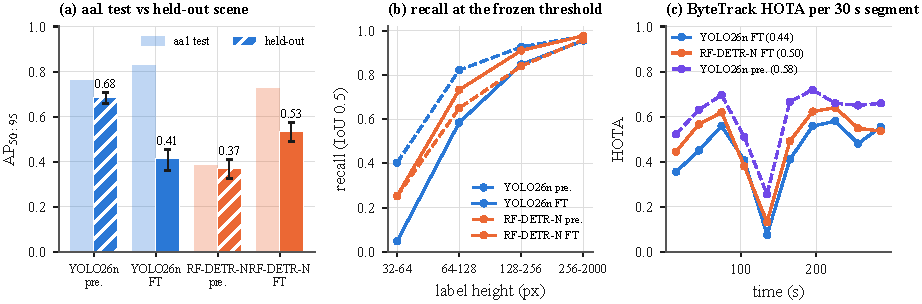
\includegraphics[width=\textwidth]{figures/fig_heldout.pdf}
\caption{Held-out video (test only). (a) \AP{} on the aa1 test split (light) and on the held-out video (dark, 95\%
block-bootstrap CI); hatched: COCO-pretrained. (b) Recall by label height at the thresholds frozen from aa1.
(c) ByteTrack HOTA per 30\,s segment with the aa1 parameters (whole-video HOTA in the legend); the dip near 135\,s is a
stretch with almost nobody in view.}
\label{fig:heldout}
\end{figure*}}

\textbf{Tracking and analytics.} With the frozen parameters, fine-tuned \rfdetr{} tracks better than fine-tuned \yolo{}
(Table~\ref{tab:hotrack}): it wins \HoSegWinsRf{} of \HoSegs{} 30\,s segments (Wilcoxon $p=\HoSegPFtFt$) and
\HoTcWinsRf{} of \HoTcPairs{} tracker$\times$GT combinations of the six-tracker comparison, the reverse of aa1. The
pretrained \yolo{}, never tuned for tracking, is best and wins \HoSegWinsPt/\HoSegs{} segments against \rfdetr{}
($p=\HoSegPPtRf$). Absolute HOTA (\HoBtHotaYoloFtTun--\HoBtHotaYoloPtTun{} vs.\ \BtHotaYoloTun{} and \BtHotaRfTun{} on the aa1 hold-out) is depressed by distant people that the
students do not detect: mean occupancy is \HoAnOccYoloFt, \HoAnOccRfFt{} and \HoAnOccYoloPt{} vs.\ \HoAnGtOcc{} in the
pseudo-GT. Near the camera the analytics are more robust: the pretrained \yolo{} recovers the counting-line events
with F1 \HoAnCrossFoneYoloPt{} (count error \HoAnCrossErrYoloPt). Unique-ID counts are not a usable metric here:
\rfdetr{} reports \HoAnUniqueRfFt{} people vs.\ \HoAnGtUnique{} in the pseudo-GT only because track fragmentation
(\HoBtIdswRfFtTun{} ID switches) and missed distant people cancel.
\ifHaveHeldoutEdge
The deployed runtime with the fine-tuned \yolo{} ONNX model inherits the detector's weakness: HOTA
\HoEdHotaHiSOne{} at the full rate (offline: \HoEdRefHota), \HoEdHotaHiSFour{} at 15\,fps and \HoEdHotaMidSFour{} with
the $544{\times}960$ Jetson input. This test also exposed a runtime bug that the constant-rate aa1 video could not:
without an explicit output rate, FFmpeg's raw-video output resampled the variable-frame-rate file to a constant rate
(\HoVfrDelivered{} instead of \HoVfrFrames{} frames), and file timestamps computed as index\,/\,mean fps drifted by up
to \HoVfrTsErr\,s. Frames are now passed through unchanged and stamped with their container timestamps; this raised
the full-rate HOTA from \HoVfrHotaBefore{} to \HoEdHotaHiSOne{} and left every aa1 number unchanged.
\fi
\fi
